\section{Results}
In the following, we present the results of testing various properties of our model in UPPAAL. Our findings are then compared to the results from the algorithm paper's experiments, which were originally conducted in a python script using Pygame \parencite{AlgorithmPaper}.

\subsection{Property testing}
\subsubsection{Sanity checks and alignment}
Before diving into the actual data, we designed a number of UPPAAL queries to test whether our system behaved as expected. These include queries such as \texttt{Pr[<=10000](<> allDone) >= 0.98}, which tests whether the robots all reach the terminal state within a large time bound, and \texttt{Pr[<=10000]([] allDone imply sameCycle) >= 0.98}, which determines whether all robots are in the same cycle when the robots reach the terminal state. Both of these return that the property holds, i.e. that this happens with probability $>98\%$. Even if this number is not technically a guarantee, UPPAAL has not been able to produce a counterexample in the thousands of runs that we have done. Our inspection of the algorithm and these tests align on the expectation that the robots should always reach a consensus and terminate, and that the robots are in the same cycle when this happens. Additionally, we created tests for assuring that the options in the decision space, Q, were equally likely to end up as the network consensus. With the query \texttt{Pr[<=30000; 1000](<> allDone \&\& (decision[0] == 0))} we were able to determine that no matter the size of Q, the probability of selecting decision 0 as the consensus was always $1/n$.
\newline
\newline
The Lee and Liu experiment with the effects of a number of various parameters, namely the network topology and size, and the number of decicision from which the robots can choose. In the following sections, we run similar tests to compare our model against the more idealized results from the original article \parencite{AlgorithmPaper}. We defer this comparison to section 8.


\subsubsection{Effects of network topology}
\begin{table}[h!]
\centering
\begin{tabular}{|l|c|c|c|}
\hline
\textbf{Topology Experiment} & \textbf{Network Size} & \textbf{Number of Options} & \boldmath$D_{\text{rel}}$ \\
\hline
Original (\cite{AlgorithmPaper}) & 30 robots     & 30 options   & 0.22 - 0.43 \\
\text{Our Experiment}    & \text{30 robots} & \text{30 options} & \text{0.22 - 0.43} \\
\hline
\end{tabular}
\caption{Comparison of experimental designs for testing the effects of network topology}
\label{tab:experiment-design}
\end{table}

For the effects of network topology, we copied all of the experiment parameters. However, since the networks are randomly generated, they are never going to be exact duplicates of the original networks.
Like Lee and Liu, we run each experiment for a 100 trials and post the average in the graph below. Our exact queries can be found in appendix A.

\begin{figure}[H]
    \centering
    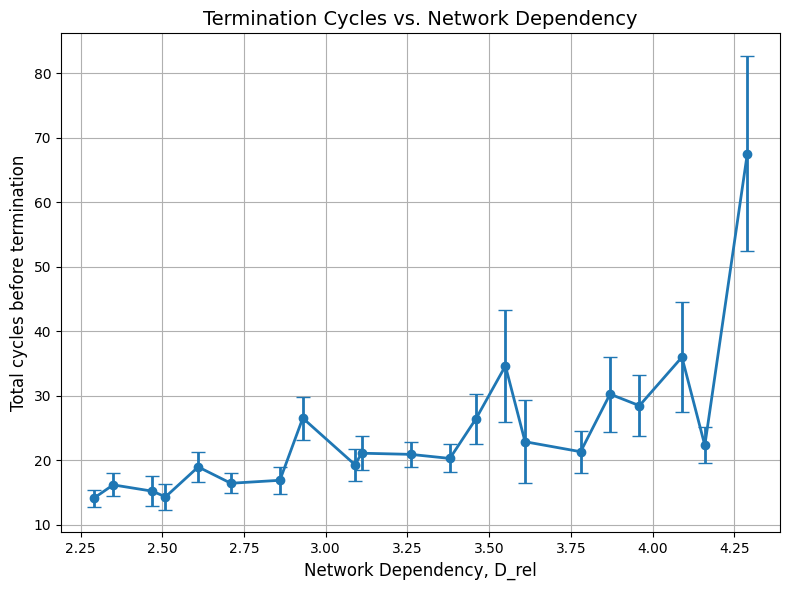
\includegraphics[width=0.9\linewidth]{pictures/DrelGraph.png}
    \caption{Results from experiments based on network dependency. The correlation between these variables have been found to have a Pearson value of 0.69}
    \label{fig:D_relResults}
\end{figure}

These variables are found to be moderately correlated with a Pearson value of 0.69 \parencite[page 1765]{pearson}. The results are statistically significant with P $<$ .00001.


\subsubsection{Effects of network size}
\begin{table}[h!]
\centering
\begin{tabular}{|l|c|c|c|}
\hline
\textbf{Network Size Experiment} & \textbf{Network Size} & \textbf{Number of Options} & \boldmath$D_{\text{rel}}$ \\
\hline
Original (\cite{AlgorithmPaper}) & 30 - 150 nodes     & 30 options   & 3.0 $\pm$ 0.1 \\
\text{Our Experiment}    & \text{5 - 50 nodes} & \text{30 options} & \text{3.0 $\pm$ 0.1} \\
\hline
\end{tabular}
\caption{Comparison of experimental designs for the effects of network size}
\label{tab:experiment-design}
\end{table}

For the effects of network size, we copied all of the experiment parameters as well as possible, but were forced to user smaller network sizes. This is imply due to how UPPAAL conducts the experiments, which becomes computationally heavy and unfeasible before the program crashes. The results, however, are still of interest.
Like before, we run each experiment for a 100 trials and post the average in the graph below. Our exact queries can be found in appendix A.

\begin{figure}[H]
    \centering
    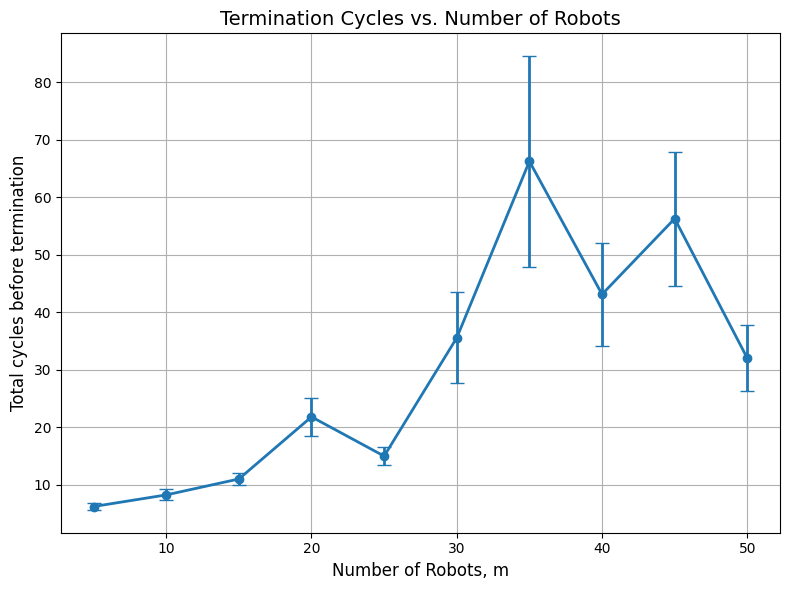
\includegraphics[width=0.9\linewidth]{pictures/RGraph.png}
    \caption{Results from experiments based on network size. The correlation between these variables have been found to have a Pearson value of 0.78}
    \label{fig:D_relResults}
\end{figure}

These variables are found to be strongly correlated with a Pearson value of 0.78 \parencite[page 1765]{pearson}. The results are statistically significant with P $<$ .00001.

\subsubsection{Effects of the size of the decision space}
\begin{table}[h!]
\centering
\begin{tabular}{|l|c|c|c|}
\hline
\textbf{Options Experiment} & \textbf{Network Size} & \textbf{Number of Options} & \boldmath$D_{\text{rel}}$ \\
\hline
Original (\cite{AlgorithmPaper}) & 30 nodes     & 10 - 300 options   & 2.672 \\
\text{Our Experiment}    & \text{30 nodes} & \text{10 - 300 options} & \text{2.675} \\
\hline
\end{tabular}
\caption{Comparison of experimental designs for the effects of option space size}
\label{tab:experiment-design}
\end{table}

For the effects of the size of the decision space, we copied all of the experiment parameters as well as possible, but due to the randomly generated networks, we had to choose a network with a 0.003 higher network dependency score. We expect that this small parameter will yield no significant change in the results.
Once again, we run each experiment for a 100 trials and post the average in the graph below. Our exact queries can be found in appendix A.

\begin{figure}[H]
    \centering
    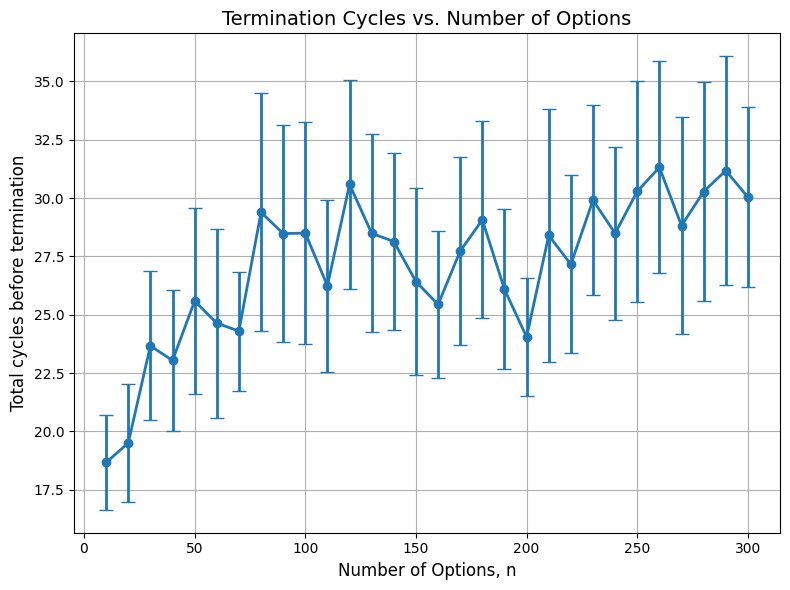
\includegraphics[width=0.9\linewidth]{pictures/QGraph.png}
    \caption{Results from experiments based on number of options. The correlation between these variables have been found to have a Pearson value of 0.73}
    \label{fig:D_relResults}
\end{figure}

These variables are found to be strongly correlated with a Pearson value of 0.73 \parencite[page 1765]{pearson}. The results are statistically significant with P $<$ .00001.

\subsubsection{Effects of the size of external interference}
Lee and Liu additionally run a number of experiments on the effects of seeding \parencite{AlgorithmPaper}. Seeding is meant as the act of predetermining the preferred decision of a number of robots. The effects of these seeds robots on the final outcome are then observed.
The details for the original experiment \parencite{AlgorithmPaper} are somewhat unclear. For example, there is no mention of the network dependency value of the networks or the size of the decision space. For our experiments, we will be using a randomly generated network of 30 robots with a network dependency value of 2.84. We set the number of options to 30, and predetermine the seed robots to exhibit a preference of 13\% for the first option at index 0, with the remaining options each having a 3\% preference. This spread can be largely influential, and no precedence is set in the original paper. Consequentially, the results should be interpreted as such.

\begin{figure}[H]
    \centering
    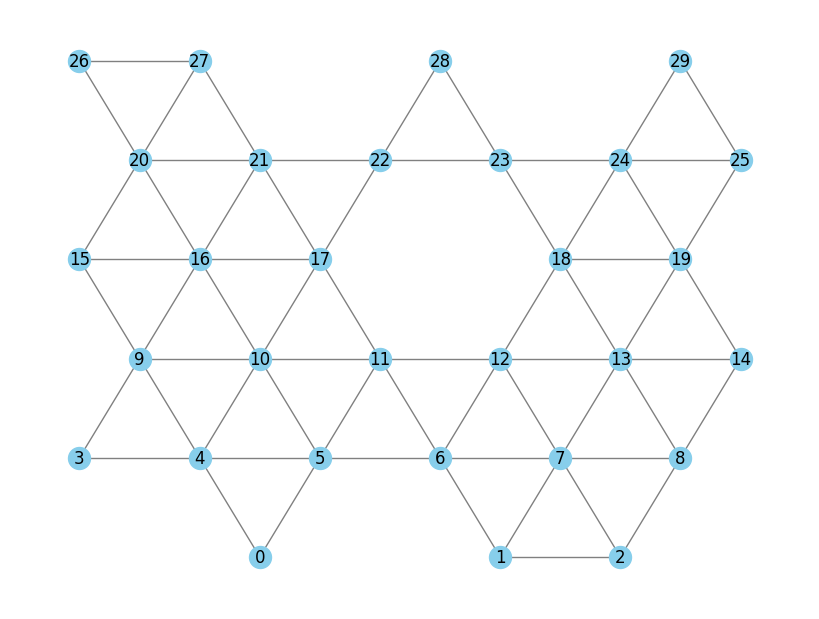
\includegraphics[width=0.9\linewidth]{pictures/30robs.png}
    \caption{Network of 30 robots for testing the effects of seeding.}
    \label{fig:D_relResults}
\end{figure}

We initially run our queries with no seeding. In the simulations, 3/100 runs end up with consenting on decision 0, and UPPAAL estimates the probability of selecting this decision to be between about $4.6\% \pm 4\%$. This is all in line with the expected value of $1/n$.  We then run a number of simulations, and get the following results.
\begin{figure}[H]
    \centering
    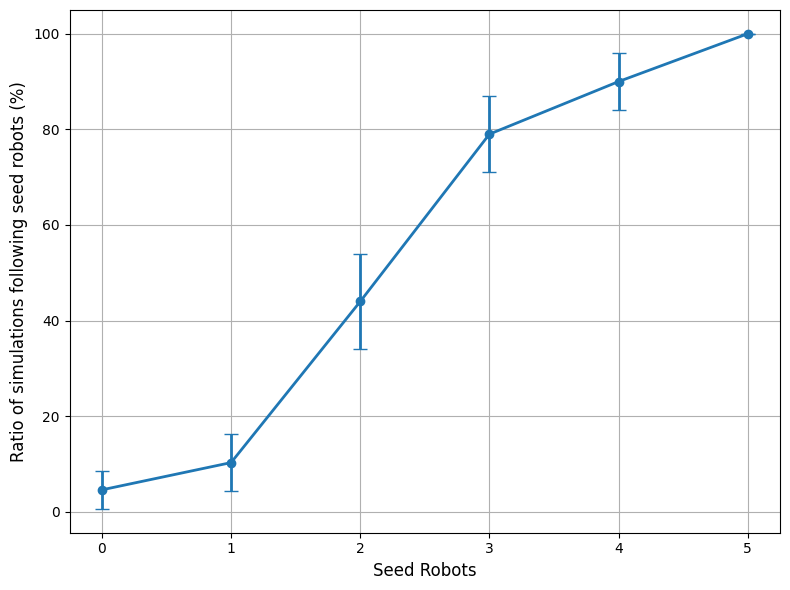
\includegraphics[width=0.9\linewidth]{pictures/SeedGraph.png}
    \caption{Effects of seeding on network consensus}
    \label{fig:D_relResults}
\end{figure}
From 5 seed robots and onward, the network always consents on the seeded decision.
%With a single seed robot, this probability jumps to $10.3\% \pm 6\%$, and at two seed robots, the probability leaps to $44\% \pm 10\%$. At three, $79\% \pm 8\%$, four, $90\% \pm 6\%$, at 5 robots and onward, the
\newline
We discuss these results in the following section.